%
% Bilderserie zur Diractfunktion
%
\begin{figure}
\centering
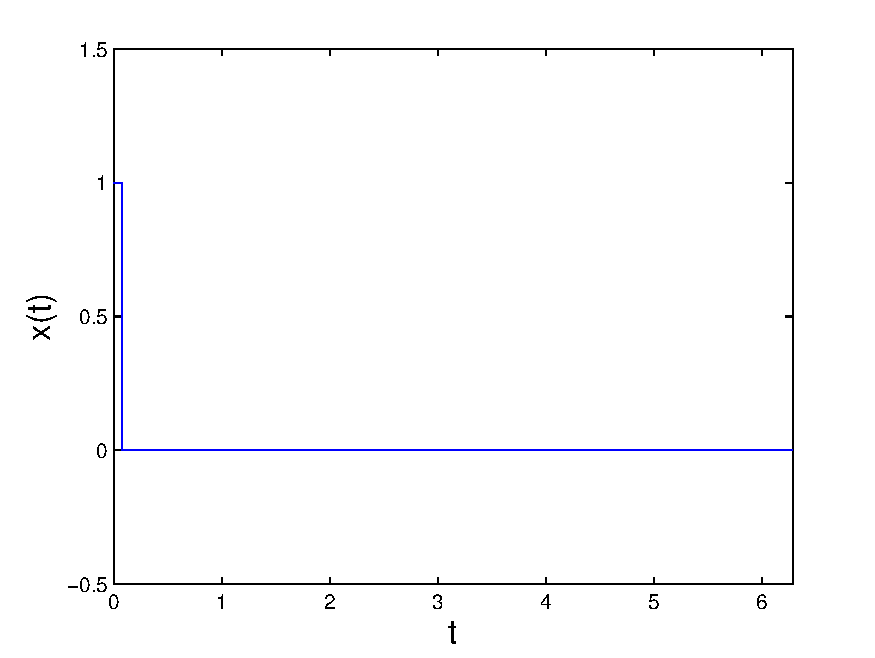
\includegraphics[width=0.45\textwidth]{kugel/Dkonstant/Rechteck1_1.pdf}
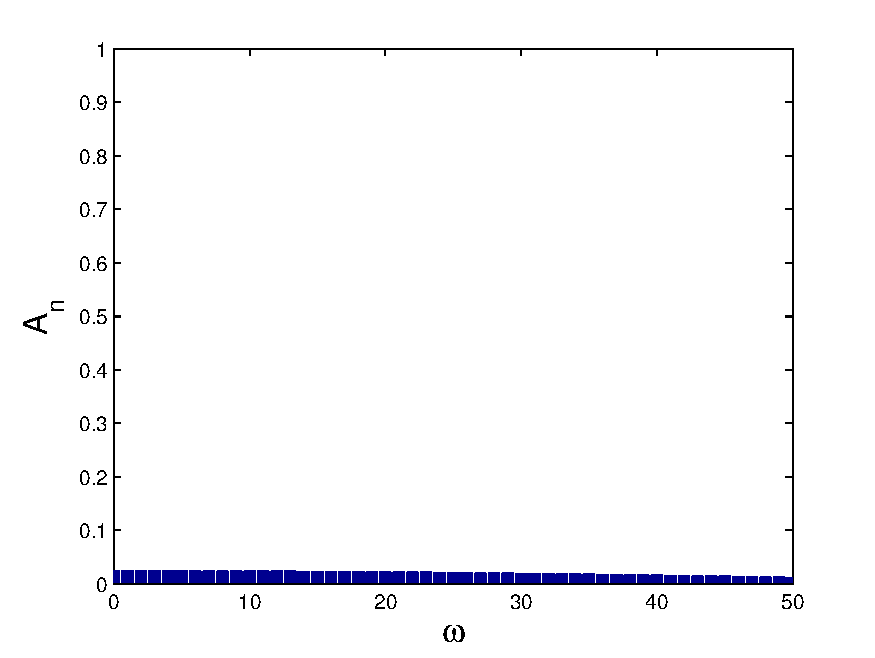
\includegraphics[width=0.45\textwidth]{kugel/Dkonstant/Rechteck1_2.pdf}
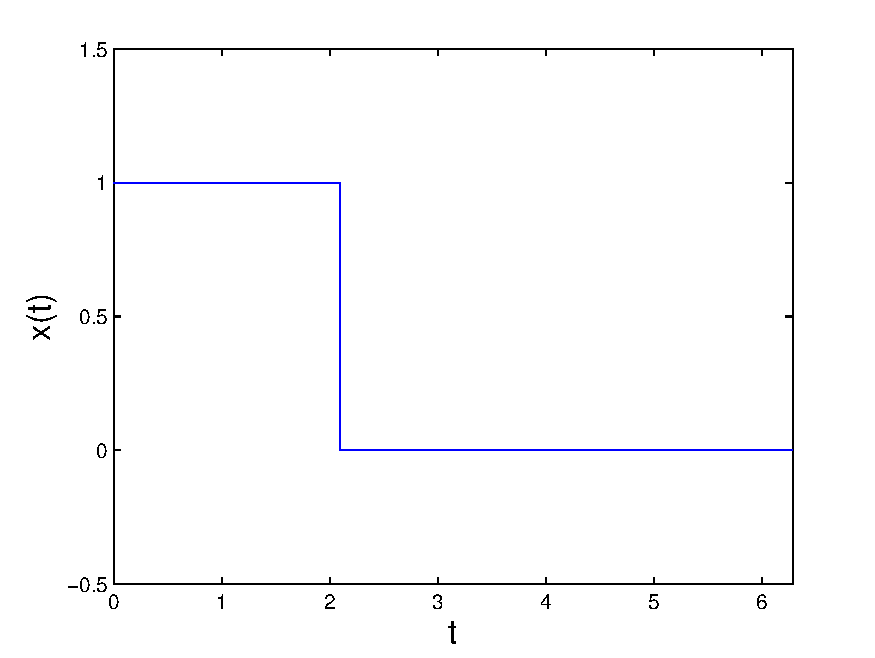
\includegraphics[width=0.45\textwidth]{kugel/Dkonstant/Rechteck2_1.pdf}
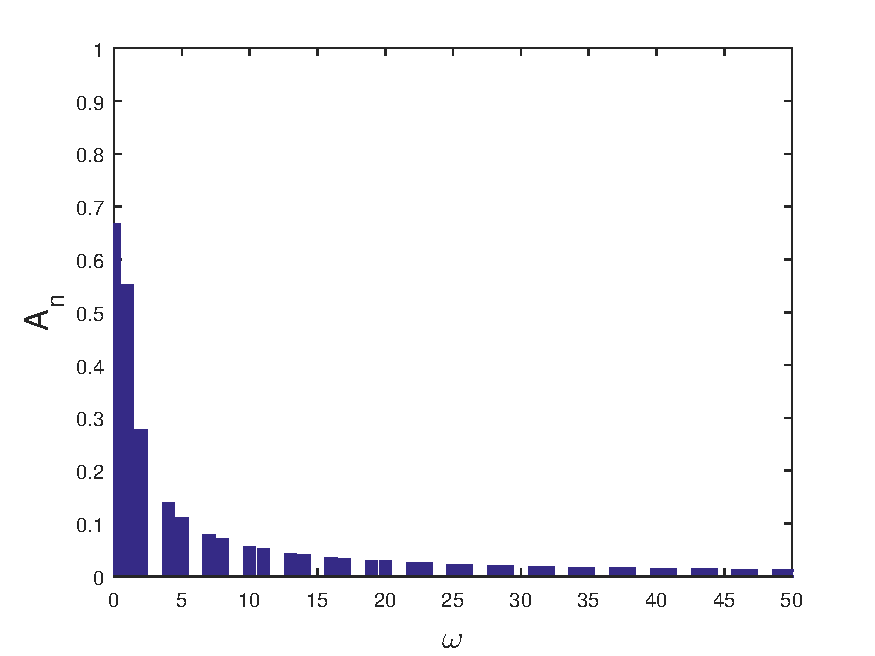
\includegraphics[width=0.45\textwidth]{kugel/Dkonstant/Rechteck2_2.pdf}
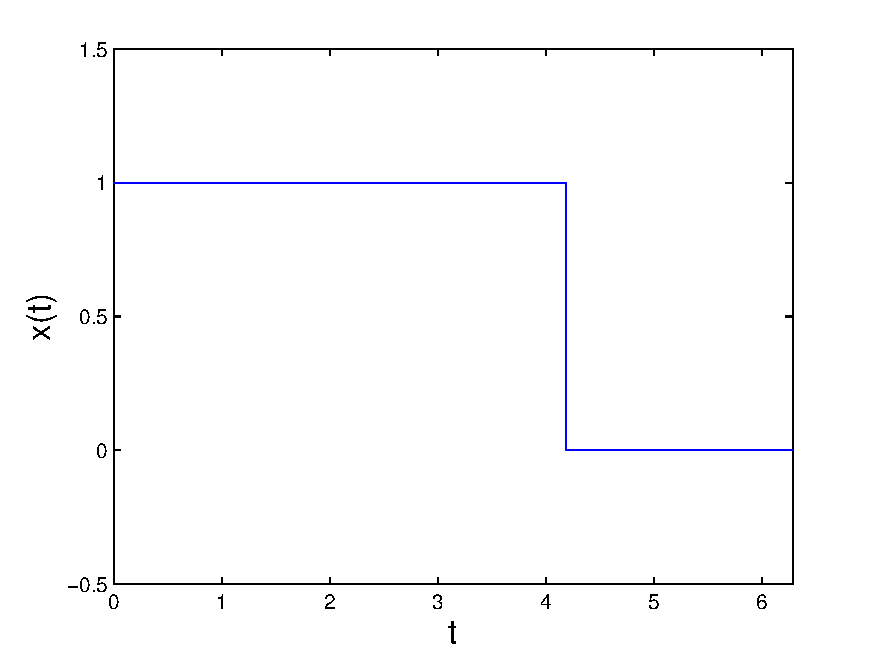
\includegraphics[width=0.45\textwidth]{kugel/Dkonstant/Rechteck3_1.pdf}
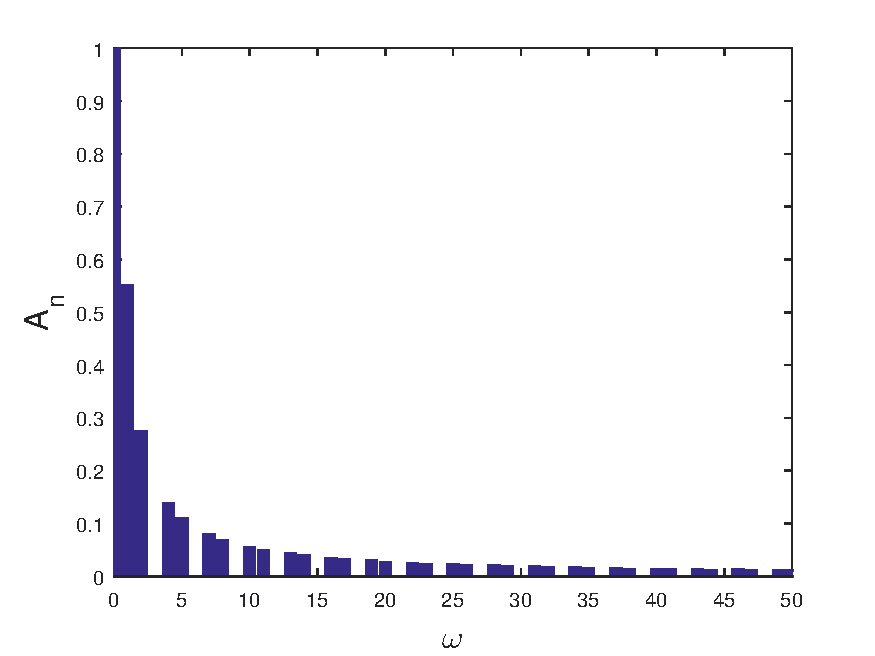
\includegraphics[width=0.45\textwidth]{kugel/Dkonstant/Rechteck3_2.pdf}
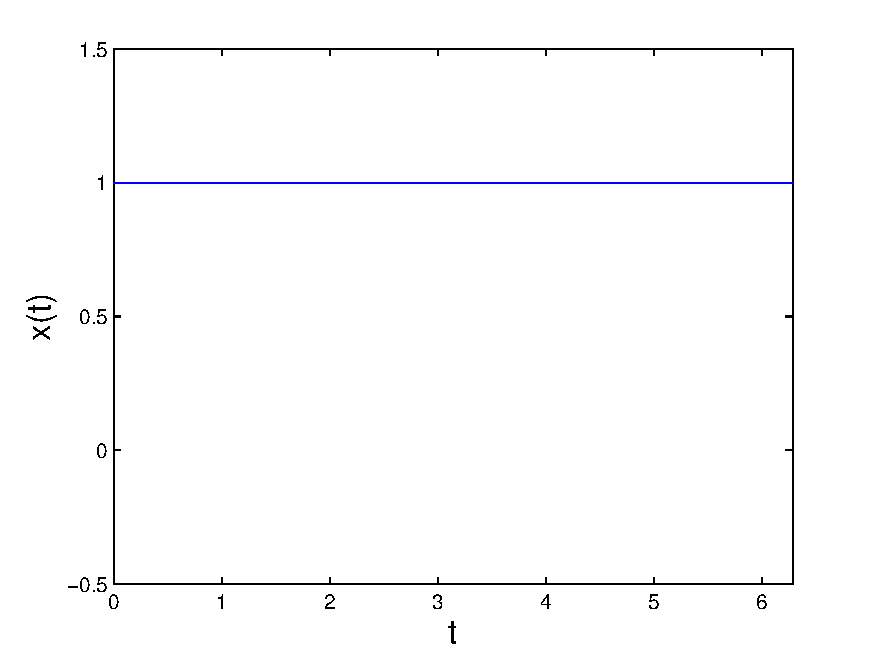
\includegraphics[width=0.45\textwidth]{kugel/Dkonstant/Rechteck4_1.pdf}
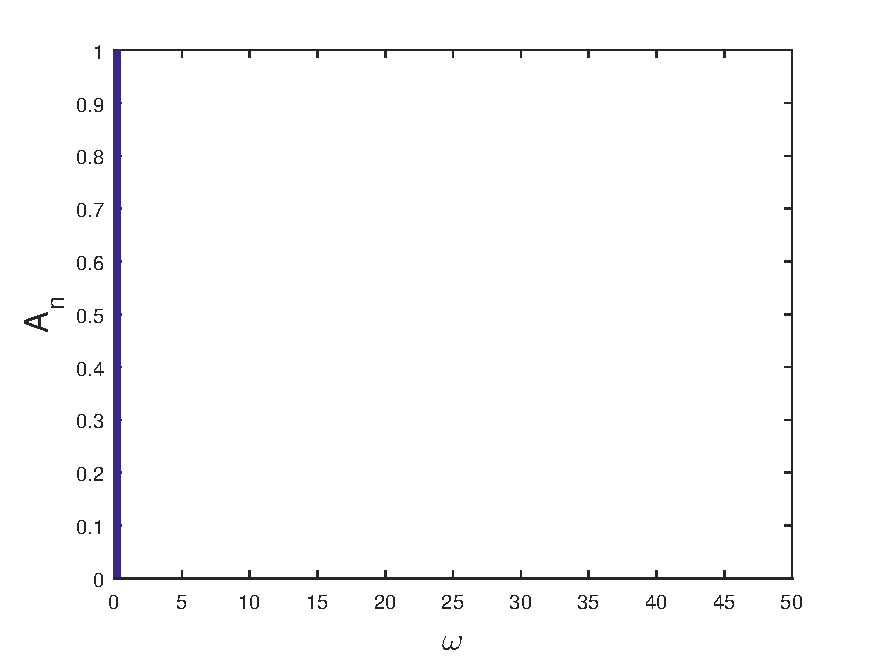
\includegraphics[width=0.45\textwidth]{kugel/Dkonstant/Rechteck4_2.pdf}
\caption{Breiter werdende Rechteckfunktion
\label{skript:Dirac1}}
\end{figure}
\begin{figure}
\centering
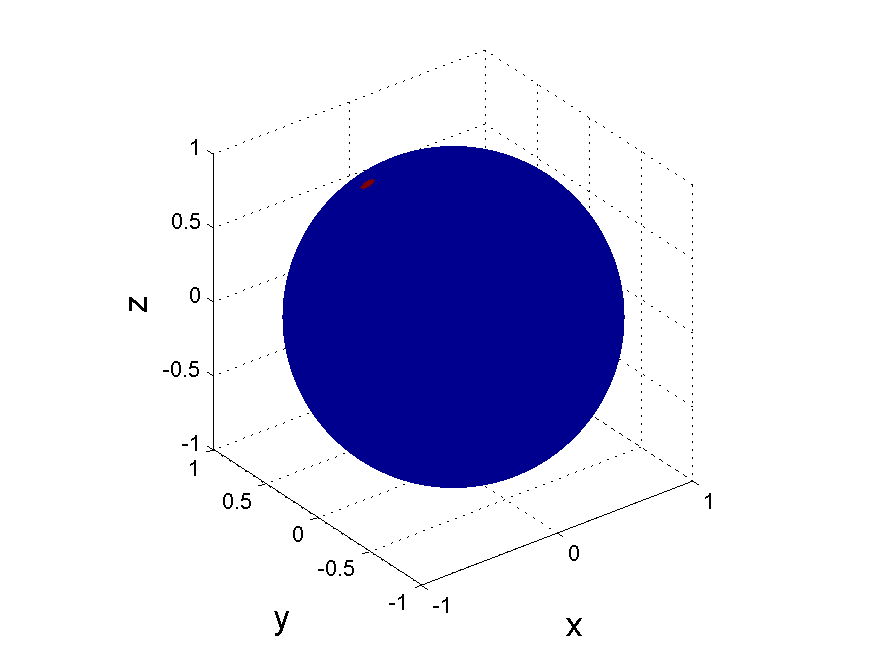
\includegraphics[width=0.45\textwidth]{kugel/Dkonstant/Kugel1_1.pdf}
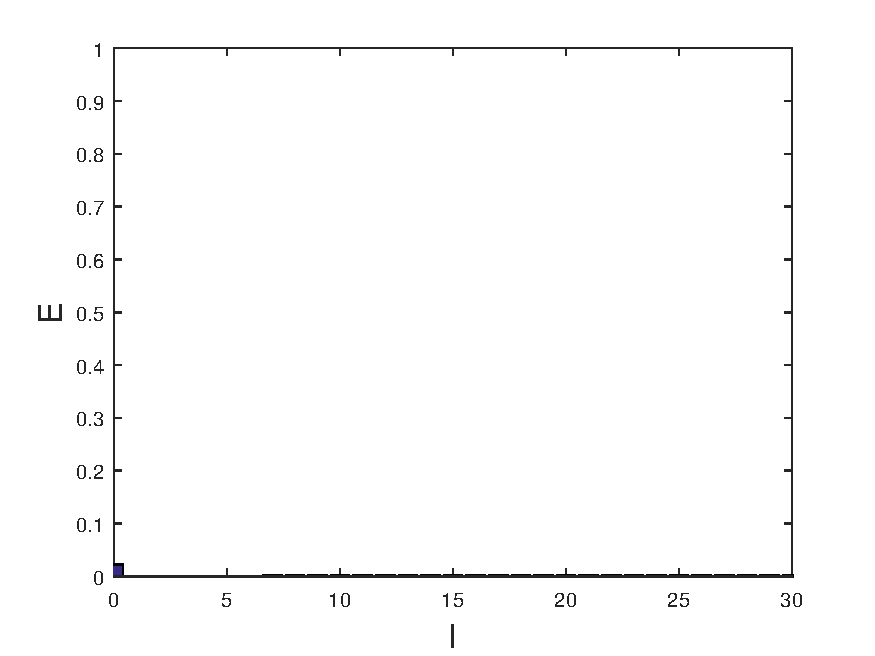
\includegraphics[width=0.45\textwidth]{kugel/Dkonstant/Kugel1_2.pdf}
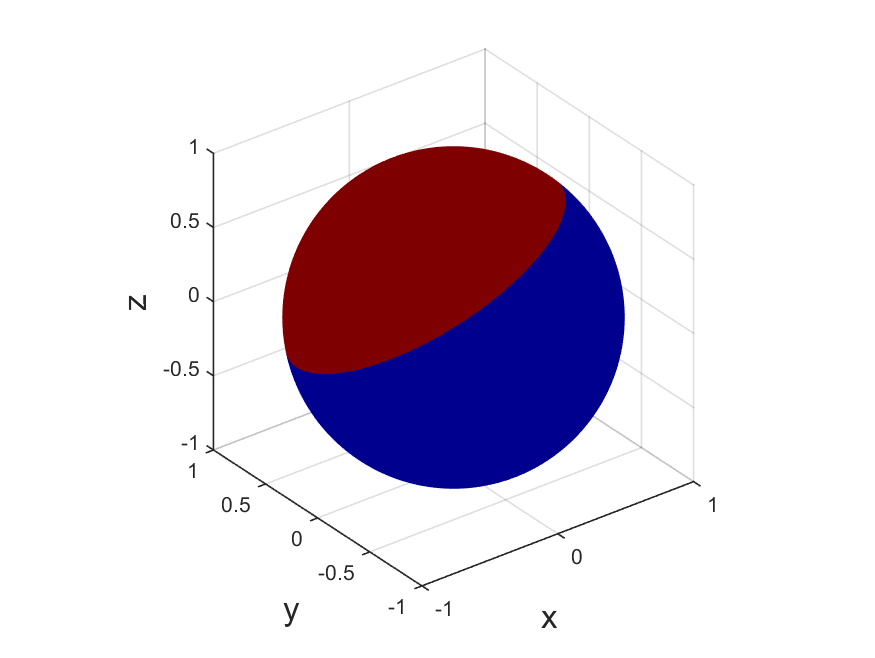
\includegraphics[width=0.45\textwidth]{kugel/Dkonstant/Kugel2_1.pdf}
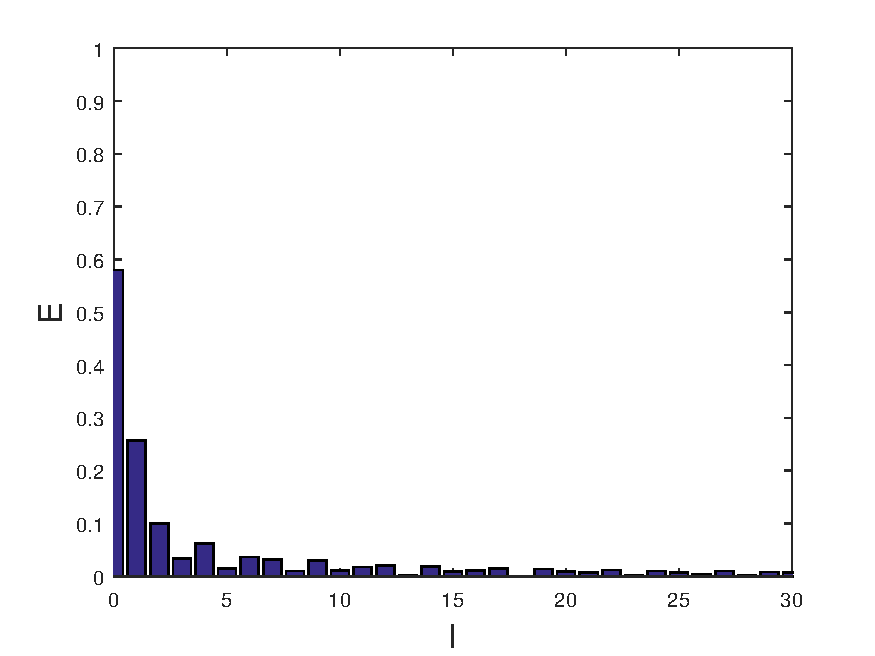
\includegraphics[width=0.45\textwidth]{kugel/Dkonstant/Kugel2_2.pdf}
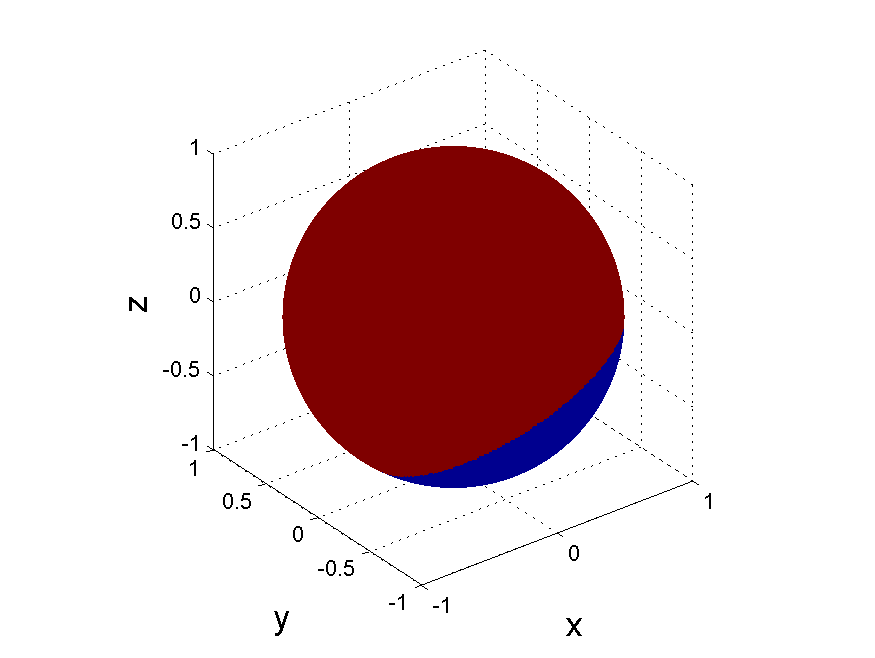
\includegraphics[width=0.45\textwidth]{kugel/Dkonstant/Kugel3_1.pdf}
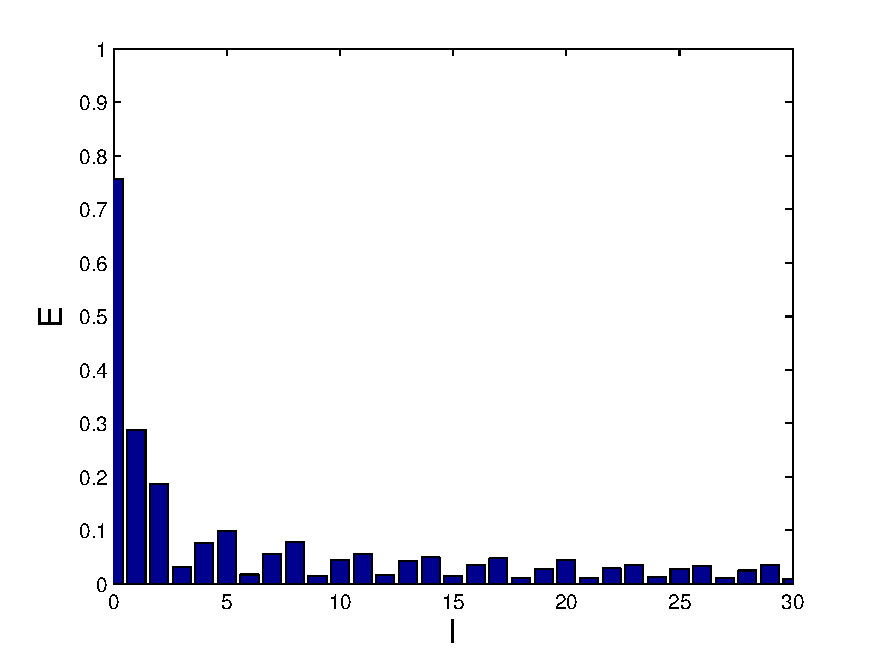
\includegraphics[width=0.45\textwidth]{kugel/Dkonstant/Kugel3_2.pdf}
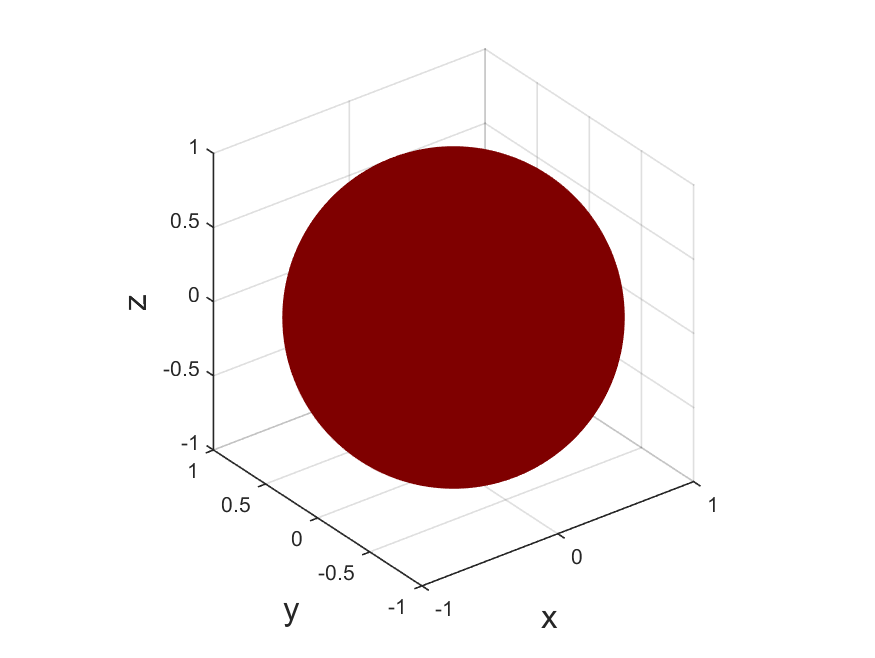
\includegraphics[width=0.45\textwidth]{kugel/Dkonstant/Kugel4_1.pdf}
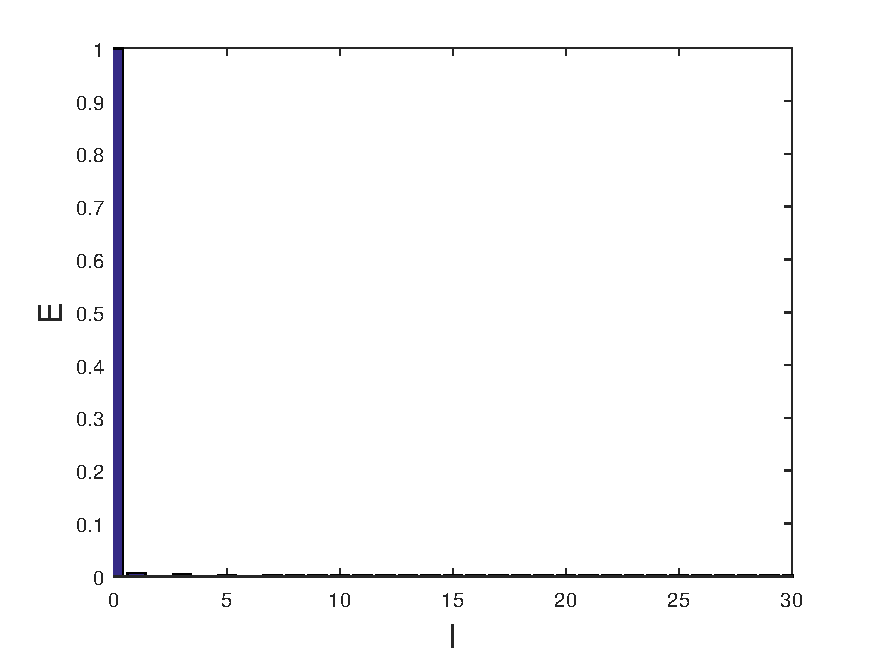
\includegraphics[width=0.45\textwidth]{kugel/Dkonstant/Kugel4_2.pdf}
\caption{Wachsender Kreisabschnitt auf der Kugeloberfl"ache
\label{skript:Dirac2}}
\end{figure}
